\chapter{Red Black Tree}
A red-black tree is a special type of binary search tree with one extra bit of storage per node, its color which can be either red or black. Also, we keep the tree approximately balanced by enforcing some properties on the tree.
\begin{definition}{Perfect Binary Tree}{}
	It is a Binary Tree in which every internal node has exactly two children and all leaves are at the same level.
\end{definition}
\begin{Lemma}{}{}
	Every perfect binary tree with $k$ leaves has $2k-1$  nodes (i.e. $k-1$ internal nodes).
\end{Lemma}
\begin{definition}{Red Black Tree}{}
	\begin{minipage}{0.5\textwidth}
		A red-black tree is a binary tree with the following properties:
		\begin{itemize}
			\item Every internal node is key/NIL node. Every leaf is a ``NIL'' node.
			\item Each node (NIL and key) is colored either red or black.
			\item  Root and NIL nodes are always black.
			\item Any child of a red node is black.
			\item The path from root to any leaf has the same number of black nodes.
		\end{itemize}
	\end{minipage}\hfill
	\begin{minipage}{0.49\textwidth}
		\centering
		\usetikzlibrary{trees,arrows,positioning, calc}
		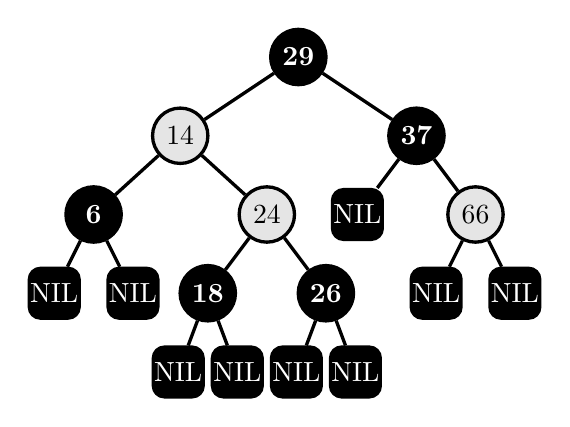
\begin{tikzpicture}[very thick,
				level/.style={sibling distance=30mm/#1},
				level distance=10mm,
				redVertex/.style={draw,fill=black!10!white,circle,minimum size=20pt,inner sep=0pt},
				blackVertex/.style={draw,fill=black,   circle,minimum size=20pt,inner sep=0pt, text=white, font=\bfseries},
				nil/.style={draw,fill=black,rectangle,rounded corners, minimum size=18pt,inner sep=0pt, text=white}]
			\node [blackVertex] (r){29}
			child {
					node[redVertex] {14}
					child [sibling distance=22mm] {
							node[blackVertex] {6}
							child {node [nil] {NIL}}
							child {node [nil] {NIL}}
						}
					child [sibling distance=22mm] {
							node [redVertex] {24}
							child [sibling distance=15mm] {
									node [blackVertex] {18}
									child {node [nil] {NIL}}
									child {node [nil] {NIL}}
								}
							child [sibling distance=15mm] {
									node [blackVertex] {26}
									child {node [nil] {NIL}}
									child {node [nil] {NIL}}
								}
						}
				}
			child {
					node[blackVertex] {37}
					child {node [nil] {NIL}}
					child {
							node [redVertex] {66}
							child {node [nil] {NIL}}
							child { node [nil] {NIL}}
						}
				};
		\end{tikzpicture}
		\captionof{figure}{A Red Black Tree}
		\label{fig:red-black-tree}
	\end{minipage}
\end{definition}

We call the number of black nodes on any simple path from  but not including a node $x$ down to a leaf the \emph{black-height} of the node, denoted by $bh(x)$. We generally confine our interest to the internal nodes of a red-black tree, since they hold the key values.
\begin{Lemma}{}{}
	A Red-Black Tree with $n$ internal nodes or key nodes has height at most $O(\log n)$.
\end{Lemma}
\begin{proof}
	We will first show that for any subtree rooted at node $x$ contains at least $2^{bh(x)}-1$ internal nodes. We will show this using induction on the height of the tree. For the base case let height of $x$ is $0$. Then $x$ must be a leaf. Therefore, the subtree rooted at $x$ has at least $bh(x)=0$. Hence, $2^{bh(x)}-1=2^0-1=0$  nodes which is true. For inductive step let $x$ has some positive height, and it is an internal node of the R-B Tree. Now $x$ has two children. Hence, each child has black-height either $bh(x)$ or $bh(x)-1$. By inductive hypothesis, the subtrees rooted at the children of $x$ have at least $2^{bh(x)-1}-1$ internal nodes. Thus, subtree rooted at $x$ has at least $2^{bh(x)-1}-1+2^{bh(x)-1}-1+1=2^{bh(x)}-1$ internal nodes.

	Now if the R-B tree has height $h$. Then any path from the root to a leaf at least half the nodes including the root must be black. So $bh(\emph{root})\geq \frac{h}2$. Thus, $n\geq 2^{\frac{h}2}-1\implies h\leq 2\log(n+1)$. Hence, we have the lemma.
\end{proof}
\nt{
	\begin{minipage}{0.3\textwidth}
		\centering
		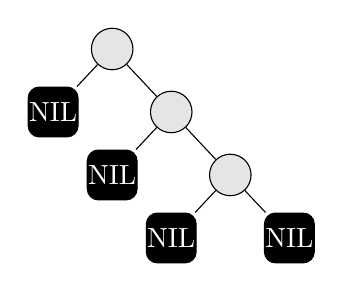
\begin{tikzpicture}[
				level distance=8mm,
				vertex/.style={draw,fill=black!10!white,circle,minimum size=15pt,inner sep=0pt},
				nil/.style={draw,fill=black,rectangle,rounded corners, minimum size=18pt,inner sep=0pt, text=white}
			]
			\node[vertex] (a) {}
			child { node [nil] {NIL} }
			child {
					node [vertex] (b) {}
					child { node [nil] {NIL} }
					child {
							node [vertex] (c) {}
							child { node [nil] {NIL} }
							child { node [nil] {NIL} }
						}
				};
		\end{tikzpicture}
	\end{minipage}\hfill
	\begin{minipage}{0.69\textwidth}
		Not all trees can be colored in a way that satisfies the properties of a red-black tree. Consider the following tree:\parinn

		In this example the root has to be black. The other two internal nodes can not be black since otherwise the path from the leaf of the root to root has only 2 black nodes but in the path from bottom most leaf to root will have 3. Then those two internal nodes has to be red. But that violates the property that a red node can not have a red child. Hence, this tree can not be colored in a way that satisfies the properties of a red-black tree.
	\end{minipage}
}
